\documentclass[12pt, a4paper]{article}
\usepackage{graphicx, xcolor, amsmath, amssymb, fontawesome, xspace, braket}
\usepackage[a4paper, left=1.5cm, right=1.5cm, top=1.5cm, bottom=1.5cm]{geometry}
\definecolor{DarkRed}{rgb}{0.76, 0.23, 0.13}
\definecolor{DarkGreen}{rgb}{0.01, 0.75, 0.24}
\definecolor{DarkBlue}{rgb}{0.47, 0.62, 0.8}
\definecolor{DarkOrange}{rgb}{1.0, 0.55, 0.0}

\begin{document}

\pagestyle{empty}
\noindent\begin{minipage}[c]{0.31\linewidth}\noindent PENDRAGON\end{minipage}\hfill
\begin{minipage}[c]{0.31\linewidth}\centering 07/04/2025 \end{minipage}\hfill
\begin{minipage}[c]{0.31\linewidth}\hfill Licence \end{minipage}\hfill

\noindent\begin{minipage}[c]{0.31\linewidth}\noindent Arthur\end{minipage}\hfill
\begin{minipage}[c]{0.31\linewidth}\hfill(2 étudiants)\end{minipage}
\begin{center} Physique -- CC\bigskip

{\Large\bf \fbox{Note: 4/5}}\end{center}

\vspace*{-0.7cm}\noindent Classement: 1\hfill Classe:  $\left(2.8 \pm 1.2\right)$/5
\noindent\rule{\linewidth}{.7pt}\begin{center}{\large\bf Détail de la note}\end{center}

\begin{center}
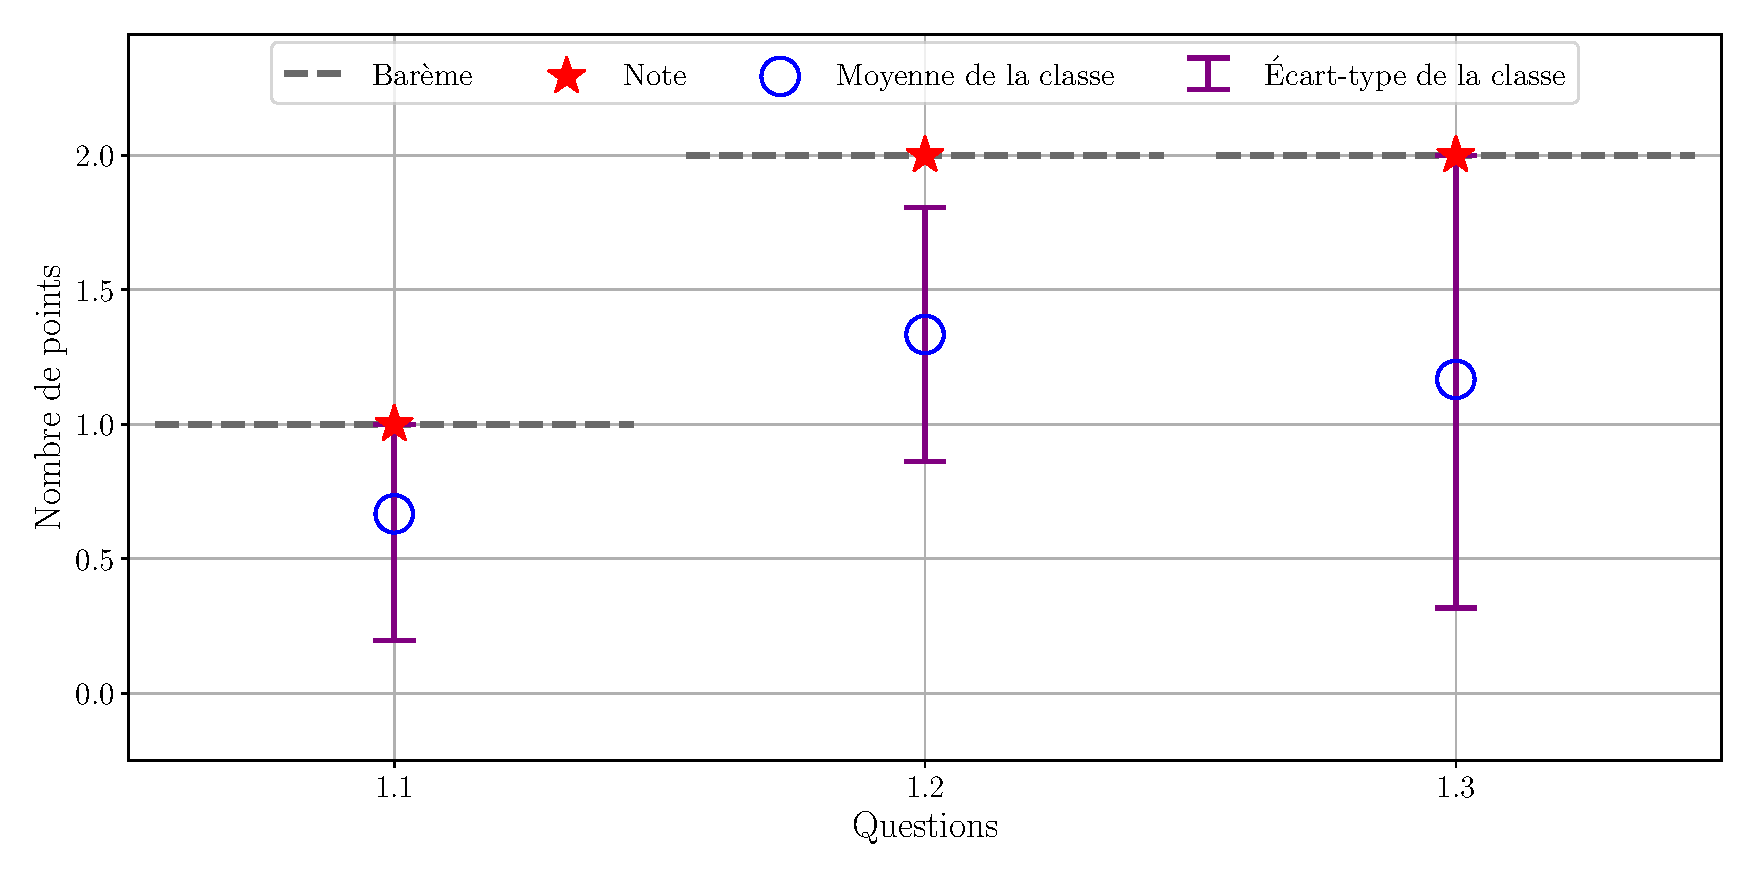
\includegraphics[keepaspectratio, width=\linewidth]{/home/abigot/effm/tutorials/output/PENDRAGON_Arthur_GradeStats.pdf}\end{center}


\noindent\rule{\linewidth}{.7pt}\begin{center}{\large\bf Remarques générales}\end{center}

$\triangleright$\xspace Aha

$\triangleright$\xspace Test


\noindent\rule{\linewidth}{.7pt}\begin{center}{\large\bf Remarques sur la copie}\end{center}

\begin{center}
\noindent \mbox{Soin\xspace\xspace\color{DarkRed}\faFrownO\color{black}}\hfill \mbox{Mise en évidence des résultats\xspace\xspace\color{DarkOrange}\faMehO\color{black}}\hfill \mbox{Numérotation des pages\xspace\xspace\color{DarkGreen}\faSmileO\color{black}}\hfill 
\end{center}


\noindent\rule{\linewidth}{.7pt}\begin{center}{\large\bf Compétences exigibles}\end{center}

\begin{minipage}[c]{0.4\linewidth}\centering
Skill number 1\xspace\xspace\color{DarkOrange}\faMehO\color{black}
\end{minipage}\hfill
\begin{minipage}[c]{0.4\linewidth}\centering
Skill number 2\xspace\xspace\color{DarkRed}\faFrownO\color{black}
\end{minipage}
\newpage
\pagestyle{empty}
\noindent\begin{minipage}[c]{0.31\linewidth}\noindent LE GAULOIS\end{minipage}\hfill
\begin{minipage}[c]{0.31\linewidth}\centering 07/04/2025 \end{minipage}\hfill
\begin{minipage}[c]{0.31\linewidth}\hfill Licence \end{minipage}\hfill

\noindent\begin{minipage}[c]{0.31\linewidth}\noindent Provençal\end{minipage}\hfill
\begin{minipage}[c]{0.31\linewidth}\hfill(2 étudiants)\end{minipage}
\begin{center} Physique -- CC\bigskip

{\Large\bf \fbox{Note: 1.5/5}}\end{center}

\vspace*{-0.7cm}\noindent Classement: 2\hfill Classe:  $\left(2.8 \pm 1.2\right)$/5
\noindent\rule{\linewidth}{.7pt}\begin{center}{\large\bf Détail de la note}\end{center}

\begin{center}
\includegraphics[keepaspectratio, width=\linewidth]{/home/abigot/effm/tutorials/output/LE GAULOIS_Provençal_GradeStats.pdf}\end{center}


\noindent\rule{\linewidth}{.7pt}\begin{center}{\large\bf Remarques générales}\end{center}

$\triangleright$\xspace Poursuivez vos efforts !


\noindent\rule{\linewidth}{.7pt}\begin{center}{\large\bf Remarques sur la copie}\end{center}

\begin{center}
\noindent \mbox{Soin\xspace\xspace\color{DarkOrange}\faMehO\color{black}}\hfill \mbox{Mise en évidence des résultats\xspace\xspace\color{DarkRed}\faFrownO\color{black}}\hfill \mbox{Numérotation des pages\xspace\xspace\color{DarkGreen}\faSmileO\color{black}}\hfill 
\end{center}


\noindent\rule{\linewidth}{.7pt}\begin{center}{\large\bf Compétences exigibles}\end{center}

\begin{minipage}[c]{0.4\linewidth}\centering
Skill number 1\xspace\xspace\color{DarkRed}\faFrownO\color{black}
\end{minipage}\hfill
\begin{minipage}[c]{0.4\linewidth}\centering
Skill number 2\xspace\xspace\color{DarkRed}\faFrownO\color{black}
\end{minipage}
\newpage

\end{document}